\documentclass[10pt]{iopart}
\usepackage{latexsym}
\usepackage{graphicx}
\usepackage{iopams}
\usepackage{color}

%\usepackage {amsmath}
%\usepackage {amssymb}
%\usepackage {amsfonts}
%\usepackage {amsthm}
%\usepackage {mathrsfs}
%\usepackage {natbib}
%\usepackage {latexsym}
%\usepackage {graphicx}
%\usepackage {dsfont}
%\usepackage {times}
%\usepackage {txfonts}
%\usepackage {rotating}
%\usepackage {wasysym}
%\usepackage {multirow}
%\usepackage {hhline}
\usepackage{hyperref}
%\usepackage {color}
\usepackage{bm}
%\usepackage{appendix}
\usepackage{acronym}
%\usepackage{dcolumn}   % needed for some tables
\usepackage{url}
\usepackage[normalem]{ulem}   % temporal one in draft.
\usepackage{xspace}

%\usepackage{harvard}
\usepackage{amsopn} % for using DeclareMathOperator

% variable shortcuts 
\newcommand{\Hub}{H_{0}}
\newcommand{\DL}{D_{\mathrm{L}}}
\newcommand{\lam}{\bm{\lambda}}
%\newcommand{\data}{\bm{d}}
%\newcommand{\sigpar}{\bm{\theta}}
%\newcommand{\nuispar}{\bm{\lambda}}
%\newcommand{\globpar}{\bm{\gamma}}
%\newcommand{\model}{\mathcal{H}}

\newcommand{\curlH}{\mathcal{H}}
\newcommand{\gws}{\tilde{h}}

%% ----- input git-version tag
\input{tag.tex}

\newcommand{\dcc}{LIGO-PXXXXXXXX}
\newcommand{\cm}[1]{\textcolor{red}{CM: #1}}
\newcommand{\MP}[1]{\textcolor{blue}{MP: #1}}
\newcommand{\lw}[1]{\textcolor{green}{LW: #1}}

\DeclareMathOperator{\erf}{erf}

\begin{document}

\title{Astrophysical calibration of gravitational-wave detectors}

\author{L.~Wright$^1$, M.~Pitkin$^1$ \& C.~Messenger$^1$}
\address{$^1$ SUPA, School of Physics and Astronomy, University of
  Glasgow, Glasgow G12 8QQ, United Kingdom}
\eads{\mailto{matthew.pitkin@glasgow.ac.uk}, \mailto{christopher.messenger@glasgow.ac.uk}}

\begin{abstract}
  We present an investigation into the potential of calibrating \MP{change to: ``assessing the validity of the calibration''?}
  gravitational wave detector outputs through the use of standard
  sirens. Such signals, as measured via gravitational wave
  observations provide an estimated luminosity distance which is
  subject to uncertainties in the calibration of the data.  If a host
  galaxy is identified for a given source then its redshift can be
  obtained and combined with current knowledge of the cosmological
  parameters.  This will yield the true luminosity distance and allow
  the direct comparison with the estimated value.  Discrepancies can
  then be used to correct the original calibration.~\cm{Update at end}
\end{abstract}

% acronym definitions
\acrodef{GW}[GW]{gravitational wave}
\acrodef{BNS}[BNS]{binary neutron star}
\acrodef{MWEG}[MWEG]{Milky Way equivalent galaxies}
\acrodef{BBH}[BBH]{binary black hole}
\acrodef{BNS}[BNS]{binary neutron star}
\acrodef{NSBH}[NSBH]{neutron star-black hole}
\acrodef{SNR}[SNR]{signal-to-noise ratio}
\acrodef{GRB}[GRB]{gamma-ray burst}
\acrodef{sGRB}[sGRB]{short gamma-ray burst}
\acrodef{CBC}[CBC]{compact binary coalescence}
\acrodef{EM}[EM]{electro-magnetic}
\acrodef{aLIGO}[aLIGO]{Advanced LIGO}
\acrodef{AdV}[AdV]{Advanced Virgo}

%Uncomment for PACS numbers title message
%\pacs{00.00, 20.00, 42.10}
% Keywords required only for MST, PB, PMB, PM, JOA, JOB? 
%\vspace{2pc}
%\noindent{\it Keywords}: Article preparation, IOP journals
% Uncomment for Submitted to journal title message
%\submitto{\JPA}
% Comment out if separate title page not required
\maketitle

%%%%%%%%%%%%%%%%%%%%%%%%%%%%%%%%%%%%%%%%%%%%%%%%%%
%%%%%%%%%%%%%%%%%%%%%%%%%%%%%%%%%%%%%%%%%%%%%%%%%%
\section{Introduction\label{sec:intro}}

% introduce GWs and BNS systems
It is expected that the advanced generation of interferometric \ac{GW}
detectors will detect waves emitted from $O(10s)$ of compact binary
coalescences.  One such class of these cataclysmic events, the inspiral and
merger of \ac{BNS} systems will be detected out to a maximum range of $\approx
450$ Mpc. Assuming the current best estimates for the cosmological parameters,
this is equivalent to a redshift $z\approx 0.1$. As noted by \cite{1986Natur.323..310S} \ac{CBC}
systems can be used as cosmological distance markers, otherwise known as
``standard sirens'' (analogous to the \ac{EM} standard candles). Standard sirens
allow ...

% BNS systems are GRBs
It is considered likely that the merger of \ac{BNS} systems, in addition to
emitting detectable \acp{GW}, is also the mechanism for producing \acp{sGRB}.
In this scenario these \ac{EM} events are produced through the ... and result
in tightly beamed emission parallel to the orbital angular momentum vector of
the \ac{BNS} system. Additional evidence for the coincidence of \acp{sGRB} with
\ac{GW} events are the estimated astrophysical rates of both phenomena.
Observations of \acp{sGRB} give a rate of XXX Mpc$^{-3}$yr$^{-1}$ which can be
compared to estimates of \ac{BNS} merger rates of XXX-XXX Mpc$^{-3}$yr$^{-1}$.
This latter range is obtained from population synthesis models together with
knowledge of the X known \ac{BNS} systems in our galaxy. 
  
% talk about the calibration idea
If a single \ac{GW} event is observed in coincidence with a \ac{sGRB} it will \MP{may?}
be possible to identify the host galaxy of the \ac{BNS} source.  With this
information a spectroscopic redshift can be very accurately obtained. With
knowledge of the redshift, using current best estimates for the Hubble constant
and other cosmological parameters, the true luminosity distance can be
estimated to $\sim 1\%$ accuracy.  The \ac{GW} measurement acts as a standard
siren also giving us a direct measurement of the luminosity distance to the source.
The accuracy of such a measurement depends on a number of factors including the
accuracy with which the \ac{GW} detector has been calibrated.  Hence comparison
with the distance estimate from the \ac{sGRB} we can re-calibrate (or validate)
the existing experimentally obtained calibration. 

% What do we do in this paper
In this paper we investigate the feasibility of this approach for single
coincident \ac{GW}--\ac{sGRB} events and establish the validation power of such
a calibration technique.  In Sec.~\ref{sec:calibration} we briefly summarize
the existing experimental technique for \ac{GW} detector calibration and its
expected accuracy.  We then review the concept of \ac{GW} standard sirens and
their proposed coincident \ac{EM} signatures, the \acp{sGRB} in
Secs.~\ref{sec:sirens} and~\ref{sec:GRB}. In Sec.~\ref{sec:single} we present
the results of Monte-Carlo simulations for the purpose of luminosity distance
estimation using \ac{GW} events. In Sec.~\ref{sec:cosmo} we show the likely
accuracy of \ac{sGRB} distances obtained from their host galaxy redshift and in
Sec.~\ref{sec:discussion} we conclude.    

%%%%%%%%%%%%%%%%%%%%%%%%%%%%%%%%%%%%%%%%%%%%%%%%%%
%%%%%%%%%%%%%%%%%%%%%%%%%%%%%%%%%%%%%%%%%%%%%%%%%%
\section{Gravitational wave detector calibration\label{sec:calibration}}

\cm{We need to define our model for the calibration, i.e. are we talking
about amplitude only and are we breaking this up over frequency.}

\MP{In this paper I think we stick to just talking about a single overall amplitude calibration scale.}

The technique used throughout GW research in calibrating the detectors is
carried out through a complicated system of physical manipulations of the
Fabret-Perot Michelson interferometer; where an elaborate feedback system is
used to sustain a defined measurement in arm length difference between the
moving mirrors~\cite{LIGOCal}. In general, the interferometers are set to move
at a frequency corresponding to a GW signal. An error signal is then found
through the Pound-Driver-Hall technique~\cite{Black} for mirror stabilisation
which is proportional to the difference in mirror separation of the
Fabret-Perot Michelson interferometer. The Pound-Drever-Hall technique is
essentially a control loop feedback system in which the difference output (in
GW detectors, this is the distance the mirrors move due to the GW) and the the
output set is reduced to the highest degree of certainty. This is just a brief
overview of the calibration method currently used, and is an extensive study in
itself, see \cite{Vitale:2012} and references therein. For \ac{aLIGO} and \ac{AdV},
at the frequency range used in this project, the error in the calibration using
the `hardware injection method' is roughly $10\%$ \cite{Vitale:2012}. This is a
benchmark set for the error estimation using the proposed new method in this
project.~\cm{Clean this up and expand.}

% Describe our model for the calibration
\MP{The gravitational wave strain is measured through the differential arm length, $\Delta L$, 
changes of the interferometer via $h = \Delta L(f) / L$, where $L$ is the full arm length.
Calibration is required to relate the actual measured interferometer error signal output
$e(f)$ to $\Delta L$. This relation is known as the length response function, $R(f,t)$,
defined such that
\begin{equation}
\Delta L(f) = R(f,t) e(f),
\end{equation}
where $R$ varies slowly in time (in comparison to transient signal timescales).
Calculation of $R$ requires the measurement of various functions within a control feedback loop
(see \cite{Vitale:2012} for a brief overview of this), which are subject to
uncertainties. In this study we will assume an estimate of $R$ is available (although
in theory we could take on the role of estimating $R$ itself), but that it differs from the
truth through some unknown scale factor, $s$, so that
\begin{equation}
sh(f) = h_{\rm m}(f) = \frac{R(f,t) e(f)}{L},
\end{equation}
where $h(f)$ is the true strain and $h_{\rm m}(f)$ is the measured strain. With this definition it
means that if $s > 1$ then a signal would appear to have a larger amplitude (e.g.\ be closer) than 
expected, whereas if $s < 1$ would appear to have a lower amplitude than expected. In this analysis 
we will simplify the situation by assuming that $s$ is a constant with respect to frequency, but in 
future studies that assumption could be dropped and $s$ could take some functional form, or 
piece-wise fit, with respect to $f$.}

%%%%%%%%%%%%%%%%%%%%%%%%%%%%%%%%%%%%%%%%%%%%%%%%%%
%%%%%%%%%%%%%%%%%%%%%%%%%%%%%%%%%%%%%%%%%%%%%%%%%%
\section{Binary neutron star standard sirens\label{sec:sirens}}

We should explain what this means starting with reference
to~\cite{1986Natur.323..310S}.

%%%%%%%%%%%%%%%%%%%%%%%%%%%%%%%%%%%%%%%%%%%%%%%%%%
%%%%%%%%%%%%%%%%%%%%%%%%%%%%%%%%%%%%%%%%%%%%%%%%%%
\section{GRB counterparts\label{sec:GRB}}

% what are sGRBs 
\cm{What are sGRBs?}\\

% discuss joint-event rates
\cm{Discuss the expected rate of joint detections}\\

% observing a coincident event
The most likely scenario in which a coincident \ac{GW}--\ac{sGRB} event would
be identified is through the targeted follow-up of an observed \ac{sGRB} or by
post-facto matching of \ac{GW} trigger lists with known \ac{sGRB} events.  The
likelihood of being able to follow-up \ac{GW} events using gamma-ray telescopes
with low enough latency to catch a \ac{sGRB} is low.  Compounding this issue is
the relatively large \ac{GW} sky error-box giving a field-of-view for the
\ac{EM} observatories to search spanning $\sim 100$'s of square
degrees~\cite{grb}.  For the \ac{GW} follow-up of \ac{sGRB} scenario the merger
time for \ac{BNS} systems will be estimated from the \ac{sGRB} to within a few
seconds~\cite{grb}.  This makes the follow-up search less computationally
expensive since it is performed over a smaller range of data using potentially
fewer numbers of waveform templates.  This computational saving enables the use
of a more computationally expensive multi-detector coherent scheme rather than
the cheaper coincidence methods used in the untargeted searches. 

% discuss the inclination angle issue
A fortunate consequence of a joint \ac{GW}--\ac{sGRB} observation will be the
fact that in order for such an event to be observed, the \ac{BNS} system must
have had its orbital angular momentum vector pointing towards (or away) from
the detector.  The actual inclination angle of the system, defined as the angle
between the orbital angular momentum vector and the line of sight, must be $<$
half of the \ac{sGRB} beaming angle.  This prerequisite property limits us to
systems that are approximately ``face-on'' and therefore biases us to higher
\ac{SNR} signals.  However, as discussed earlier, the property of beaming
severely impacts the probable rate of such joint observations.   


%%%%%%%%%%%%%%%%%%%%%%%%%%%%%%%%%%%%%%%%%%%%%%%%%%
%%%%%%%%%%%%%%%%%%%%%%%%%%%%%%%%%%%%%%%%%%%%%%%%%%
\section{Analysis}

\cm{This should be the simplest case we can do.  We need to cut a lot of this.}

\MP{We want to assess how well a calibration scale factor can be estimated
from a single observed \ac{GW} associated with a particular \ac{sGRB}. As we {\it a priori}
have no knowledge of the likely location and distance of such an event we have performed
simulations of multiple events to see the expected distribution the accuracy of the
calibration scale factor recovery.}

% Describe the signal model (Taylor F2 etc...)
We use the TaylorF2 waveform approximation (see e.g.\ \cite{2009PhRvD..80h4043B} and references 
therein) with a 3.5 post-Newtonian expansion in phase for modelling our signal (in both simulations 
and signal recovery).  For \ac{BNS} systems we use non-spinning waveforms under the assumption that 
spins will be negligible. For \ac{NSBH} system we use a spinning waveform, but in which only the 
black hole has non-negligible spin and that its rotational angular momentum is aligned with the 
systems orbital angular momentum.

For a non-spinning system the general form of the frequency-domain polarisation amplitudes are
%
\begin{eqnarray}\label{eq:signal}
  \gws_{+}(f) &\propto \frac{1+\cos^{2}\iota}{D_{L}}
\mathcal{M}^{5/6}f^{-7/6}e^{-i\Psi(f, \nu, t_\mathrm{c}, \phi_{\mathrm{c}})} \nonumber \\
  \gws_{\times}(f) &\propto
 \frac{\cos^{2}\iota}{D_{L}}\mathcal{M}^{5/6} f^{-7/6}e^{-i\Psi(f, \nu, t_\mathrm{c}, 
\phi_{\mathrm{c}})}
\end{eqnarray}
%
where the chirp-mass $\mathcal{M}$ is defined as $\mathcal{M}=M\eta^{3/5}$, with 
$\eta=m_{1}m_{2}/M^{2}$ and $M=m_{1}+m_{2}$, $\iota$ is the inclination angle, and $\nu=(\pi 
Mf)^{1/3}$.  The \ac{GW} strain measured at the $k^{\rm{th}}$ detector is then given by
%
\begin{equation}
  \label{eq:gravsig}
   \gws^{k}(f) = \big[ F_{+}^{k}(\alpha, \delta, \psi)\gws_{+}(f) +
F_{\times}^D(\alpha, \delta, \psi)\gws_{\times}(f)\big]
\end{equation}
%
where $F_{+},F_{\times}$ are the antenna response functions which are dependent
upon the polarisation angle $\psi$ and the sky position of the source
$\alpha,\delta$.

% Define the detectors and the noise epoch we will be using
For this analysis we will consider advanced generation instruments operating
at their design sensitivity, \MP{with noise power spectral densities taken from
\cite{2013arXiv1304.0670L}}. The network we consider is the 3 detector H1--L1--V1 configuration. 

% Define the likelihood function we will be using
We consider that the measured data in any detector is defined as
%
\begin{equation}
  \tilde{d}_{k}(f)=\tilde{n}_{k}(f)+s\gws_{k}(f,\btheta)
\end{equation}
%
where $\tilde{n}(f)$ is the Fourier transform of Gaussian noise drawn from a
distribution consistent with the power-spectral-density of the advanced
detector noise. 

\subsection{Method}

\MP{Our aim is to estimate the marginal posterior probability distribution function (pdf)
for the unknown calibration scale factors. We use Bayes' theorem for which we need to define
a likelihood function and prior pdfs on the signal parameters being estimated. In this
analysis we use the Markov chain Monte Carlo code {\tt emcee} \cite{2013PASP..125..306F} to sample 
the posterior distribution.} We use a Gaussian likelihood function given by
%
%\begin{equation}
%  p(\vec{d} | \vec{\theta}, \curlH, I) \propto \exp\Bigg[ 2\Delta
%f\sum_{k>0}\frac{|\tilde{d}(f_{k}) - \tilde{h}(f_{k})|^{2}}{S(f_{k})}\Bigg]
%\end{equation}
\begin{equation}
\fl p(\bi{d} | \btheta, \curlH, I) \propto \exp{\left[4\Delta f \sum_{k=1}^{N_{\rm det}}
  \sum_{i=i_{f_{\rm low}}}^{i_{f_{\rm high}}}\frac{\Re{\left\{ \tilde{d}^{*}_{k,i} 
\gws_{k,i}(\btheta) - \frac{1}{2}\left(\gws^*_{k,i}(\btheta)\gws_{k,i}(\btheta) + 
\tilde{d}^*_{k,i}\tilde{d}_{k,i}\right) \right\}}}{S_{k,i}}\right]}
\end{equation}
% 
where $\Delta f$ is the frequency resolution of the data, $S_k$ is the $k^{\rm th}$ detector's one 
sided noise power spectral density, and the $i$ indices increment over frequency with $i_{f_{\rm 
low}}$ and $i_{f_{\rm high}}$ corresponding to the lower and upper range in frequencies used for 
our analysis, which were 20\,Hz to 400\,Hz respectively. This frequency range was chosen as the 
vast majority of the \ac{SNR} can be found within this range, so going to lower or higher 
frequencies provides very little additional information for our analysis. The source parameters, 
and the unknown scale factor, have been subsumed into a vector $\btheta$. For a network of 
detectors, the overall likelihood function becomes a product of the likelihoods for each detectors, 
i.e.\
\begin{equation}
  \label{eq:mult-likeli}
  p(\bi{d}| \btheta, \curlH) = \prod \limits_D p(\bi{d}^D| \vec{\theta}, \curlH)
\end{equation}
where $D = \{H,L,V\}$.

\subsubsection{Prior ranges}\label{sec:priors}

The primary reason why we can use coincident observations with a GRB as a potential check of 
detector calibration is that the GRB allows us to constrain our priors on various parameters that 
would normally be highly correlated with the signal amplitude. The most important of these is that 
the GRB can provide a very tight constraint on the source distance\footnote{For \ac{BNS} and 
\ac{NSBH} systems they will be observable only in the relatively nearby Universe ($z \sim 
0.1$ and $z\sim 0.2$ for \ac{BNS} and \ac{NSBH} systems respectively), so the relation between the 
measured GRB redshift and distance is simple and our luminosity distance will be negligably 
effected by the choice of cosmology \MP{Check this?}.}. In this analysis we therefore assume that 
the source distance is known (i.e.\ has a $\delta$-function prior). Another piece of information 
that we can use from having a coincident GRB is that the system is likely to be relatively close to 
face-on (an therefore nearly circularly polarised), which allows us to place prior constraints on 
the system inclination angle. Beam opening angles for short GRBs are relatively poorly constrained 
as they are based on only a few jet break detections, however \cite{2014ApJ...780..118F} give a 
median opening angle value of $\sim 10^{\circ}$. If we assume that the beam opening angle is a 
half-normal distribution, for which the median is given by $\sqrt{2}\erf{}^{-1}(1/2)\sigma \sim 
0.67\sigma$, then a median of $\sim 10^{\circ}$ corresponds to $\sigma \sim 14.8^{\circ}$. We 
therefore place a Gaussian prior on the inclination angle with zero mean and $\sigma=14.8^{\circ}$.

Our prior on the system component masses is dependent on whether we are considering the source 
being a \ac{BNS} system or a \ac{NSBH}. For the former case the prior we use is a Gaussian 
distribution for both components with means of $1.35\,\textrm{M}_{\odot}$ and standard deviations 
of $0.13\,\textrm{M}_{\odot}$ \MP{(reference)}. In reality, for all the systems we use in our 
study, the chirp mass, which we see from equation~\ref{eq:signal} plays a role in the overall 
signal amplitude, is very well constrained by the systems phase evolution, so our prior could be 
expanded with minimal effect on the results. In the case of \ac{NSBH} systems we use the same 
prior as above for the neutron star, but for the black hole we use a prior based on the 
canonical masss distribution used for the rate results in \cite{2012PhRvD..85h2002A} with a mean of 
$5\,\textrm{M}_{\odot}$ and a standard deviation of $1\,\textrm{M}_{\odot}$. For the \ac{NSBH}
systems we also require a prior on the black hole spin (for \ac{BNS} systems we have assumed that 
the spins are small enough that they will be negligible). We use a uniform prior on the 
normalised aligned spin magnitude between $-1$ and $1$.

The final important piece of information that we can make use of from the GRB observation is the 
sky position of the source, which we take to be known precisely.

For the time of coalescence we use a uniform prior of spanning $\pm0.01$\,seconds around the 
recorded time of the signal that would be returned by the detection pipeline. For the reference 
phase a uniform prior between 0 and $2\pi$ is used, and for the polarisation angle a uniform prior 
between 0 and $\pi/2$ is used. As the signals we use are generally close to being circularly 
polarised (face-on) the phase and polarisation angle will be degenerate meaning the exact 
combination of them will have very little effect of the result.

For the spinning \ac{NSBH} systems we use a uniform prior on the dimensionless spin magnitude of 
the black hole between $-1$ and 1.

Finally, we require a prior on the calibration scale factors for each detector. We make the 
assumption that in general the calibration will be correct, so want to use a prior that is peaked 
at unity. We also assume that the probability density that the calibration scale factor is either 
larger or smaller than unity by an equivalent factor, e.g.\ $s=10$ or $s=0.1$, is the same. For this 
we therefore use a log-normal distribution as our prior
\begin{equation}
 p(s|I) = \frac{1}{s\sigma\sqrt{2\pi}}\exp{\left( -\frac{(\ln{s} - \mu)^2}{2\sigma^2} \right)},
\end{equation}
where we chose $\sigma = 1.07$, which in turn means that having the mode at unity gives $\mu = 
1.15$. With these parameters the prior probability density at 0.1 and 10 is one tenth of that at 
1. Note that this prior does not provide produce a symmetric amount of probability about unity, but 
given our simulation criterion described below in Section~\ref{sec:simulations} we find that the 
likelihood generally overwhelms the prior. As $s$ is a scale factor we also have the further 
constraint that it must be positive.

\subsection{Simulations}\label{sec:simulations}

To estimate how well we can constrain the calibration scaling for each detector in an advanced 
detector network we have performed simulations with injected \ac{BNS} and \ac{NSBH} signals at a 
range of distances (50\,Mpc to 500\,Mpc with 50\,Mpc increments for the \ac{BNS} signals and 
100\,Mpc to 1000\,Mpc with 100\,Mpc increments for the \ac{NSBH} signals). The simulations use the 
two Advanced LIGO detectors (one at Hanford -- H1 -- and one at Livingston -- L1) and the Advanced 
Virgo detector (V1). The simulations are all performed in the freqeuncy domain and span a frequency 
range from 20\,Hz to 400\,Hz. We assume all detectors are expected to be operating at their design
sensitivity (as given by Figure 1 of \cite{2013arXiv1304.0670L}). As such we add noise to each 
simulation based on the sensitivity curve, but scaled with the associated calibration scale factor.

% Describe the ensemble of simulations used
Separately for the \ac{BNS} and \ac{NSBH} systems we have performed 2000 simulations at each 
distance value. For proposing injections for each simulation the source parameters were randomly 
drawn from the prior distributions given in Section~\ref{sec:priors}, with the sky position being 
drawn randomly from a uniform distribution, and with the scaling factors for each detector drawn 
from a Gaussian distribution with a mean of one and standard deviation of $0.125$ (equivalent to a 
mean fractional offset of 10\%). However, in accepting a proposed injection as one to be analysed 
we introduced a criteria that the signal be ``detectable'', based on it having an SNR of $\geq 5.5$ 
in at least two detectors as used in \cite{2012PhRvD..85h2002A} (as these would be signals 
coincident with a GRB we do not include the often used further constraint that the total coherent 
network SNR is greater than 12). The coalescence times for all injections were held fixed 
within the centre of the prior window. This criteria means that as we go to larger distances our 
population of injected sources will not be uniformly distributed over the sky, and will generally 
be closer to being circularly polarised. For the \ac{NSBH} systems it also means that at larger 
distances we will have more sources with larger mass ratios \MP{Check this}.

These simulations allow us to assess how well on average we would be able to constrain the 
calibration scale for a given CBC-GRB coincidence.



\section{Results}\label{sec:results}

A simple assumption that one could make would be that the uncertainties on the calibration scale 
factors (if they are independent of other parameters and have a Gaussian probability distribtuion) 
should be given by $\sim 1/{\rm SNR}$ for each detector. As we will show below this assumption is 
reasonable, but correlations do exist between parameters meaning that it does not completely hold, 
especially in the case on \ac{NSBH} systems with a spinning component.

For each of the simulated sources we have used the {\tt emcee} python MCMC package to perform 
parameter estimation over the unknown source parameters using the prior as discussed in 
Section~\ref{sec:priors}. In each case we use an estimate of the noise PSD based on the design 
sensitivity, but simulated as if estimated by averaging 64 separate PSD estimates and scaled with 
the same factor as applied to the injection and noise\footnote{We do not account for there being 
a difference between the estimated PSD and the actual PSD of the analysed section of data. This 
difference would be very much correlated with the scale factor, so in reality our estimate of the 
scale factor would be a combination of the calibration offset and the difference in the PSD. As 
such our results on real data would be an upper limit on the calibration scale factor.}. This has 
provided posterior probability distributions on the calibration scale factors for each detector 
\MP{Show an example for both source types}. Examples of the marginalised posterior probabilities
for a \ac{BNS} system and a \ac{NSBH} system observed with the three detector network are shown in 
figures~\ref{fig:bnspost} and \ref{fig:nsbhpost} respectively.

From these posterior distributions we have calculated the 68\% credible region on the scale factors 
for each detector (if these were Gaussian distributions this is equivalent to the region bounded by 
$1\sigma$ intervals). For all the signals at each distance increment we have 
produced the distribution of the fractional half widths (i.e.\ $1\sigma$) of these scale factors 
confidence intervals compared to the actual value. These are shown as boxplots in 
figures~\ref{fig:bnsresults} and \ref{fig:nsbhresults} for the \ac{BNS} and \ac{NSBH} systems 
respectively. The boxes show the extent from the lower to upper quartile of the values, whilst the 
whiskers represent the range of values. The black line within each box gives the median value and 
the star gives the mean value. Also shown on each plot as the dashed magenta line is the percentage 
of proposed injections that actually fulfilled the detection criterion.

\begin{figure}
 \begin{center}
  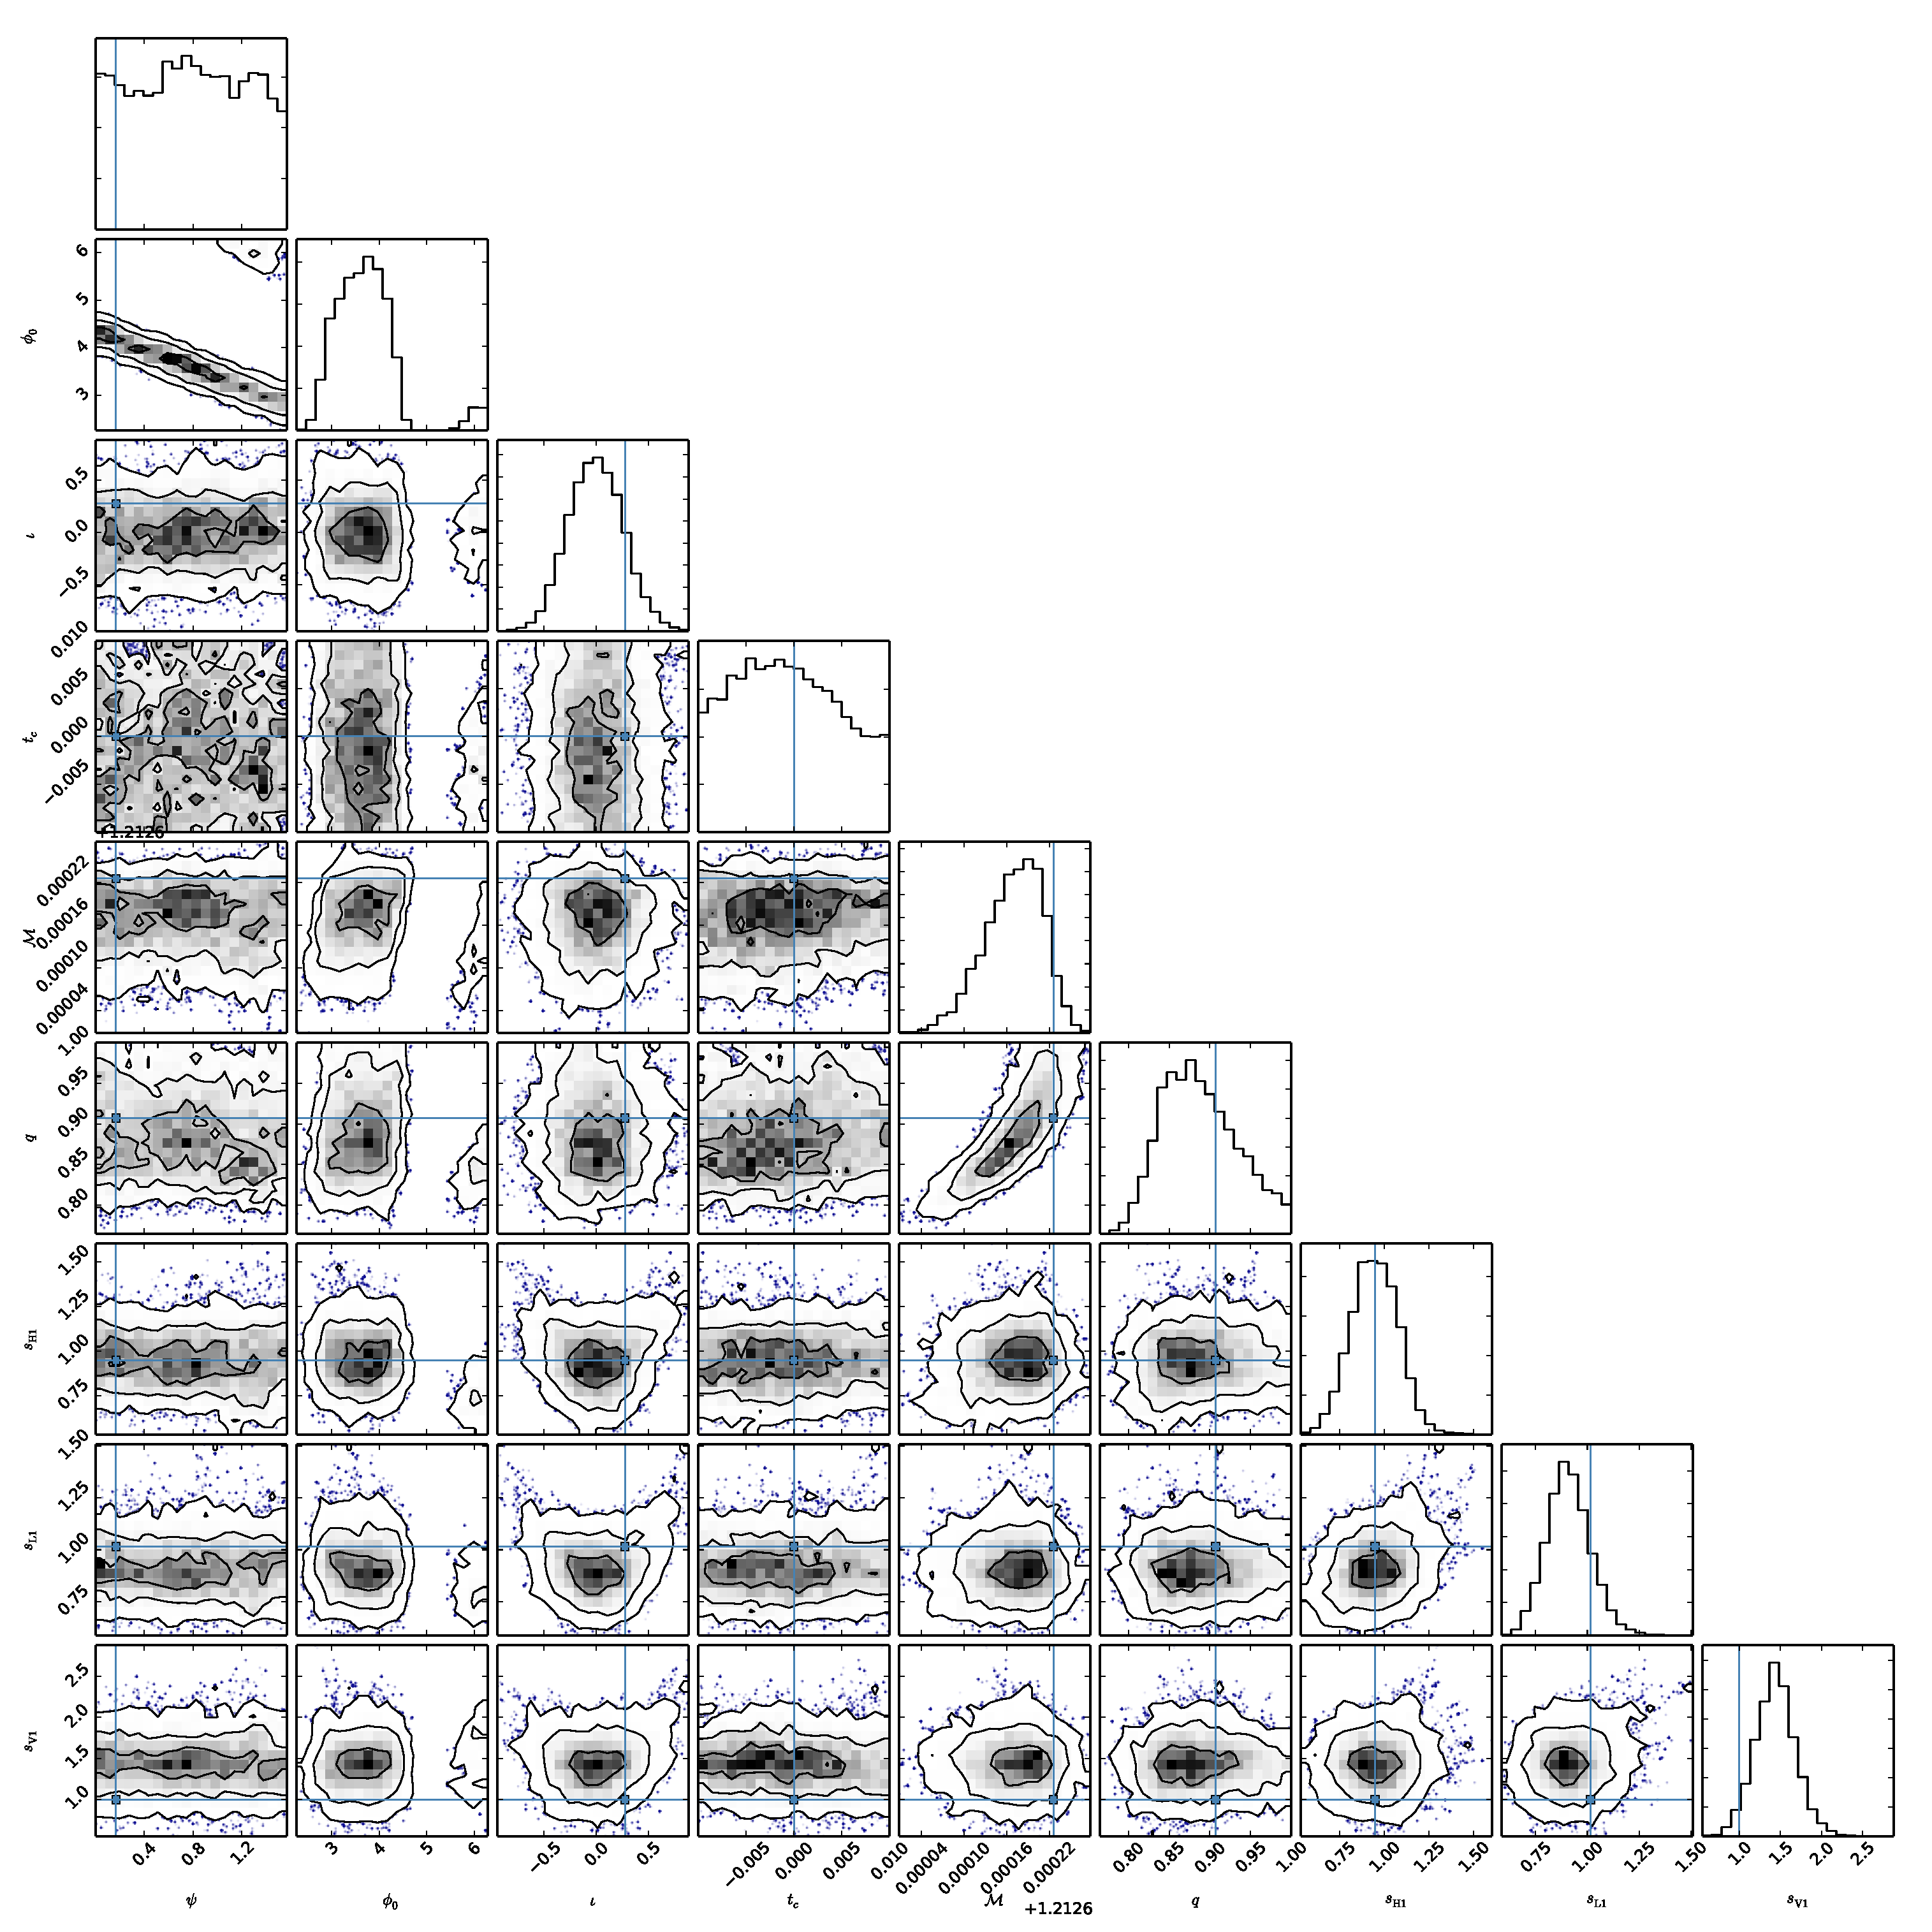
\includegraphics[width=1.0\textwidth]{bns_post_fig.pdf}
 \end{center}
 \caption{\label{fig:bnspost} The marginalised posterior probability distributions for the unknown
 parameters of a \ac{BNS} system including calibration scaling factors for the three detectors (H1, 
L1 and V1). The injected signal was at a distance of 250\,Mpc, had \ac{SNR} of 8.7, 10.9 and 4.1 
and percentage uncertainties in the calibration scale factors of 14\%, 11\% and 27\% for each of 
the detectors respectively.}
\end{figure}

\begin{figure}
 \begin{center}
  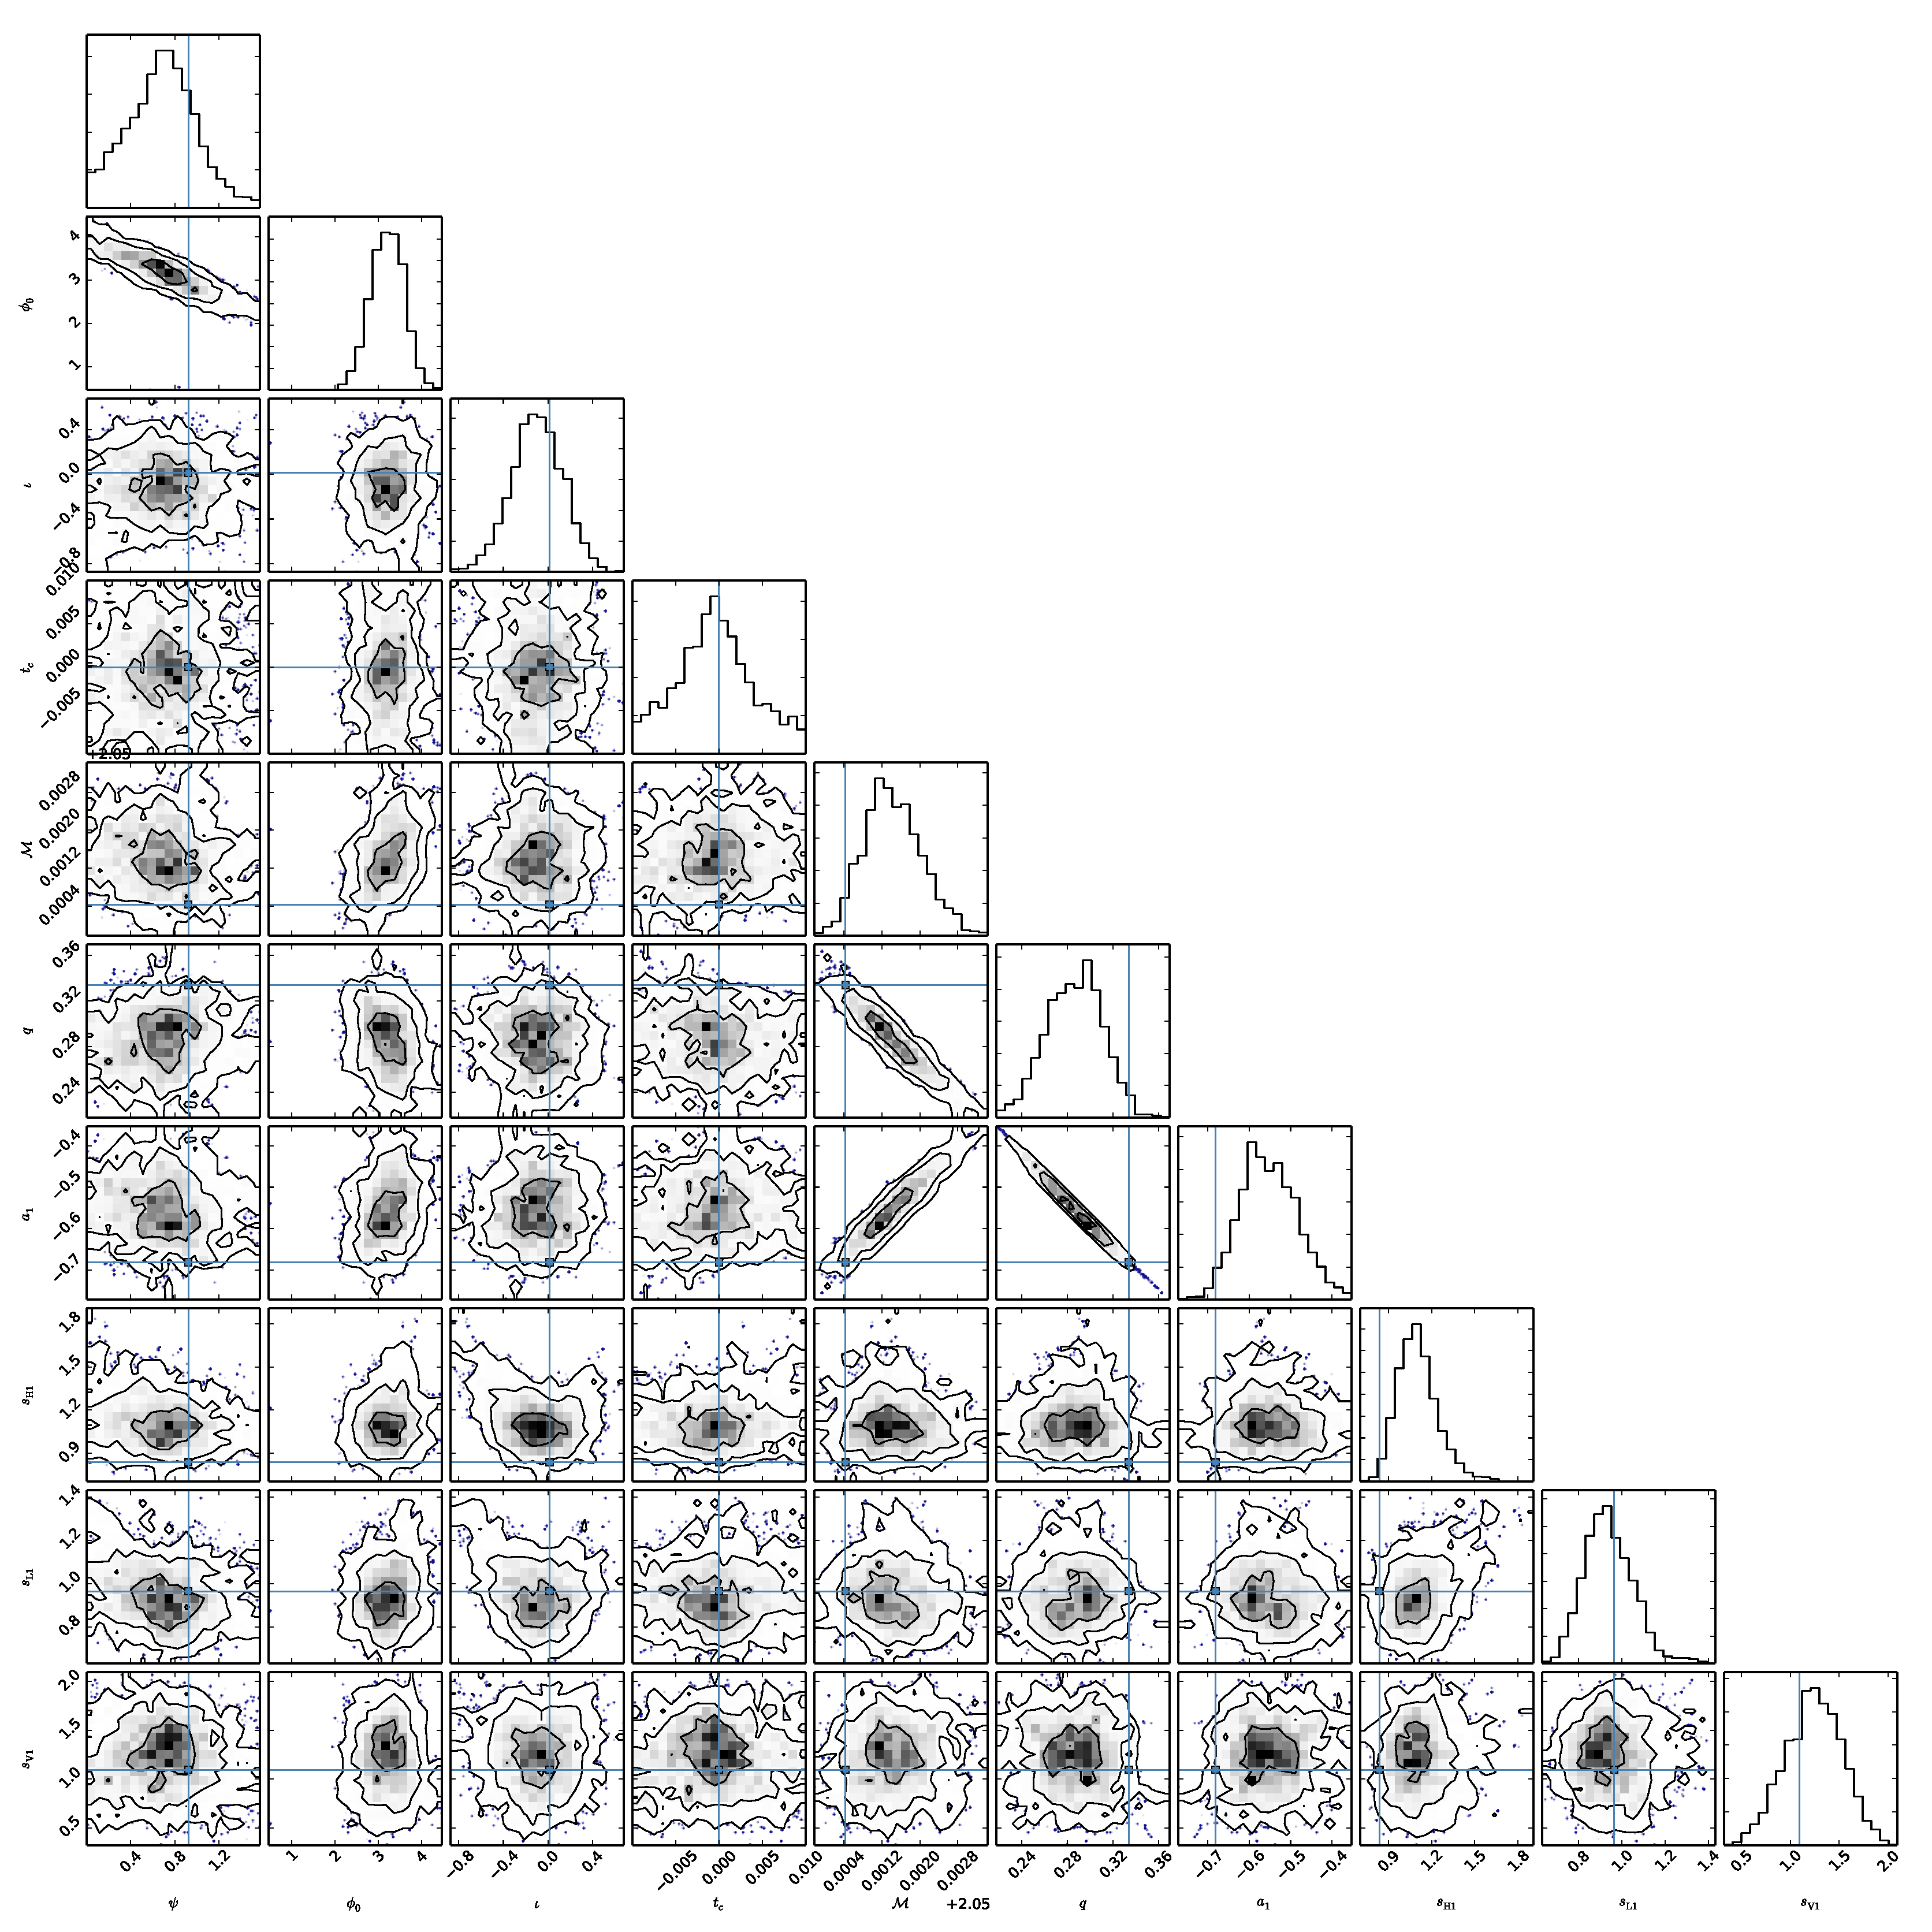
\includegraphics[width=1.0\textwidth]{nsbh_post_fig.pdf}
 \end{center}
 \caption{\label{fig:nsbhpost} The marginalised posterior probability distributions for the unknown
 parameters of a \ac{NSBH} system including calibration scaling factors for the three detectors 
(H1, L1 and V1). The injected signal was at a distance of 450\,Mpc, had \ac{SNR} of 7.7, 10.9 and 
4.2 and percentage uncertainties in the calibration scale factors of 17\%, 14\% and 34\% for each of 
the detectors respectively.}
\end{figure}

\begin{figure}
 \begin{center}
  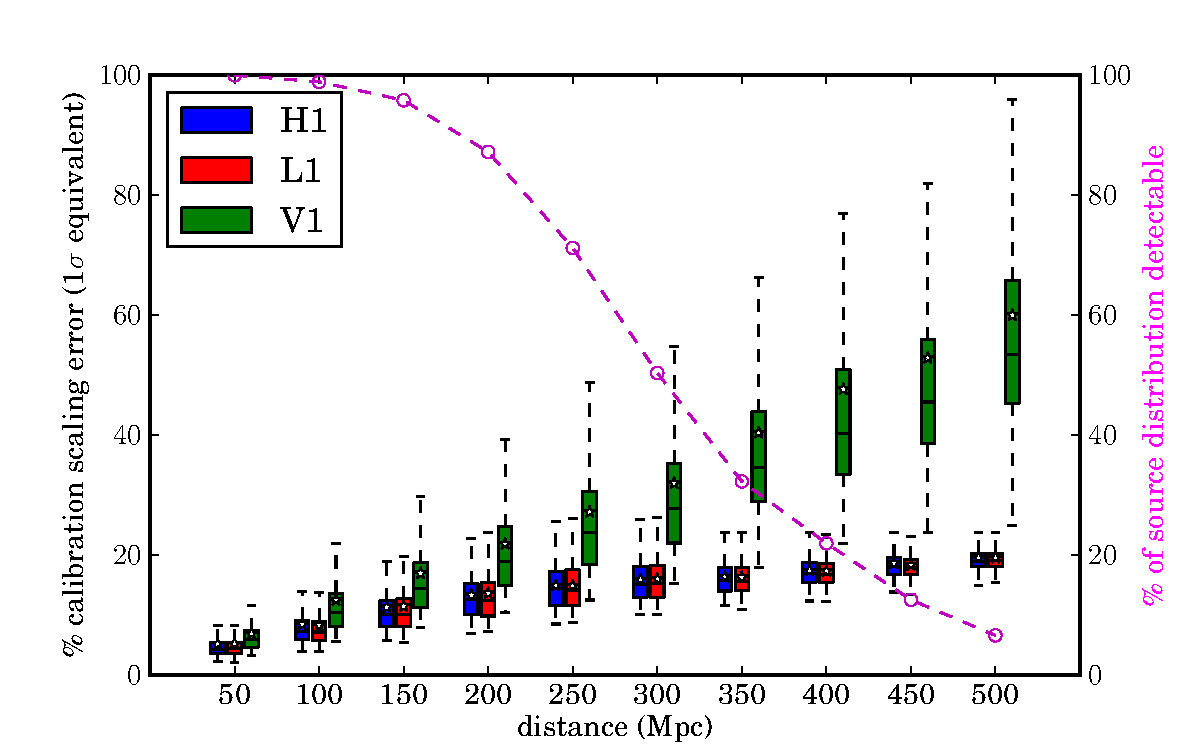
\includegraphics[width=1.0\textwidth]{scale_factor.pdf}
 \end{center}
 \caption{\label{fig:bnsresults} Distribution of the percentage accuracy at which the calibration 
scale factor can be determined for a three detector network if assuming \ac{BNS} systems (provided 
a coincident GRB is observed and can yield a distance estimate). The boxplots span the lower to 
upper quartile range of the distributions, with the median value shown as a horizontal line within 
the box and the mean shown as a star. The dashed magenta line shows the percentage of source drawn 
from the prior distribution that would be detectable at each distance value.}
\end{figure}

\begin{figure}
 \begin{center}
  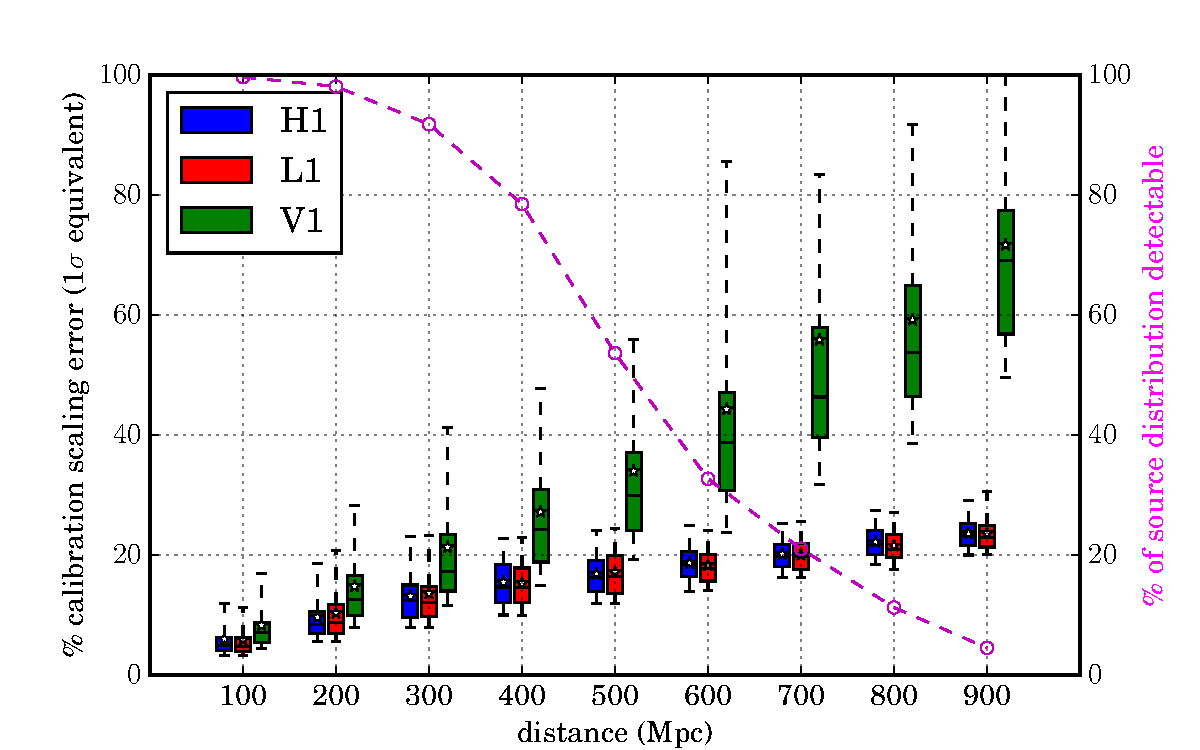
\includegraphics[width=1.0\textwidth]{scale_factor_nsbh.pdf}
 \end{center}
 \caption{\label{fig:nsbhresults} Distribution of the percentage accuracy at which the calibration 
scale factor can be determined for a three detector network if assuming \ac{NSBH} systems (provided 
a coincident GRB is observed and can yield a distance estimate). The plot contents are the same as 
in figure~\ref{fig:bnsresults}.}
\end{figure}

In figure~\ref{fig:bnsresults} we see that unsurprisingly on average the scale factor can be 
recovered to equivalent precision in both \ac{aLIGO} detectors, with uncertainties generally within 
the 10\% range for sources at 100\,Mpc. An interesting feature that we see is that for distances 
$\gtrsim 250$\,Mpc the upper extent of the uncertainty hits a maximum at $\sim 25\mbox{--}30\%$, 
whilst the width of boxes narrows. This is due to our ``detectability'' criteria, in that for all 
distances we will only be seeing those sources with high enough SNR that we would consider them 
detectable. There will therefore be fewer sources with SNR higher than this criteria at large 
distances, giving us a narrower range, and we automatically exclude those with SNR that are too 
small thus truncating our uncertainty distribution at the upper range. However, this does show that 
on average for sources that are detectable out to 450\,Mpc we would be able to constrain the 
calibration scale factor uncertainty to $\sim 20\%$. As the detection criteria will generally come 
from the SNR being high enough within the two \ac{aLIGO} instruments this means that the SNR in 
\ac{AdV} can be small and thus the ability to constrain the scale factor for it becomes poor 
(although it still provides information that the calibration is not grossly inaccurate). We also 
see that true uncertainties achievable for recovering the calibration scale factors are indeed very 
similar to the simple assumption that they would be given by $sim 1/{\rm SNR}$. Although, they are 
probably slightly poorer due to their still be correlations with $\iota$ even within the 
constrained prior range, and slight correlation between the scale factors for H1 and L1 as seen in 
figure~\ref{fig:bnspost}.

In figure~\ref{fig:nsbhresults} we see slightly different results. Despite the generally higher SNR 
for the \ac{NSBH} systems we find that on averge that the scale factor uncertainty is still roughly 
20\% at distances to 400--500\,Mpc. The range of uncertainty values is also far broader at all 
distances and there is not the plateau and upper limit seen for the \ac{BNS} systems. \MP{This 
needs checked, but ... This broader range of uncertainties appears to be down to the inclusion of 
the spin parameter and correlations this has with the mass ratio $q$ - show posterior examples. The 
lack of an upper plateau seems to be due to the detection criteria having a different effect on the 
distribution of sources that could be seen, in particular it biases the observable sources towards 
having a higher mass ratio (again check this) and thus having more correlation with the spin.}

%%%%%%%%%%%%%%%%%%%%%%%%%%%%%%%%%%%%%%%%%%%%%%%%%%
%%%%%%%%%%%%%%%%%%%%%%%%%%%%%%%%%%%%%%%%%%%%%%%%%%
\section{Distance estimates from \acp{sGRB}\label{sec:cosmo}}

~\cm{Describe the cosmological analysis used to obtain the distance from the
GRB}

%%%%%%%%%%%%%%%%%%%%%%%%%%%%%%%%%%%%%%%%%%%%%%%%%%
%%%%%%%%%%%%%%%%%%%%%%%%%%%%%%%%%%%%%%%%%%%%%%%%%%
\section{Multiple events without counterpart\label{sec:multiple}}

\cm{A discussion of the issues regarding multiple events
without EM counterparts.}

%%%%%%%%%%%%%%%%%%%%%%%%%%%%%%%%%%%%%%%%%%%%%%%%%%
%%%%%%%%%%%%%%%%%%%%%%%%%%%%%%%%%%%%%%%%%%%%%%%%%%
\section{Discussion\label{sec:discussion}}

\cm{What did we learn.}

This project is only the beginning in testing this new method of calibration.
More rigorous testing has to be carried out for a number of different systems.
As mentioned above, a larger number of random sky positions have to be analysed
to give better understanding of the resolution capabilities of the method. The
current technique of calibration defines the error in the detector to be a
complex function of frequency and phase of the GW. Instead of the simple scale
factor used so far, a more realistic error can be tested to ensure that the
estimation in its value is still comparable with current methods.


For applications of this calibration method, hypothesis testing could be
carried out. Testing different hypothesis is the technique used in determining
a GW signal in a data-set when compared to a noise-only data-set. Being able to
show with confidence that the data contains a signal is the primary focus of GW
research at the moment. Therefore if uncertainty can be removed from the
analysis this will ensure a more confident detection. Using this new method is
resolving and removing the uncertainty is an area which has to be explored.

\MP{We emphasise that our work has assumed that the PSD used in the likelihood function
when estimating the calibration scale factor is an accurate representation of the
PSD at the time of the observed CBC signal. In reality the PSD may be estimated from
a period close to, but not overlapping, the signal time and therefore may be slightly
different \cite{2013PhRvD..88h4044L}. Our result would therefore be completely correlated
with any uncertainty in the PSD estimate, but would still offer an upper limit
on the calibration uncertainty.}

\MP{The BayesLine algorithm \cite{2015PhRvD..91h4034L} may provide a natural
way to perform this analysis in particular when accounting for a frequency
dependent calibration.}

\ack

We would like to acknowledge the useful discussions with a whole bunch
of people. LW was part funded for this work through a Royal Astronomical
Society Undergraduate Research Bursary.
MP is funded by the STFC under grant number ST/L000946/1.

\section*{References}

%\biaxbliographystyle{jphysicsB}
\bibliographystyle{iopart-num}
\bibliography{masterbib}
\end{document}


